\begin{activity} \label{A:11.8.3} In each of the following questions, set up, but do not evaluate, the requested integral expression.

\ba

	\item Let $S$ be the solid bounded above by the graph of $z = x^2+y^2$ and below by $z=0$ on the unit circle. Determine an iterated integral expression in cylindrical coordinates that gives the volume of $S$.

	\item Suppose the density of the cone defined by $r = 1 - z$, with $z \geq 0$, is given by $\delta(r, \theta, z) = z$. A picture of the cone is shown in Figure \ref{F:11.8.Cylindrical_ex}, and the projection of the cone onto the $xy$-plane in given in Figure \ref{F:11.8.Cylindrical_proj}. Set up an iterated integral in cylindrical coordinates that gives the mass of the cone.
\begin{figure}[ht]
\begin{center}
\begin{minipage}{2.5in}
\begin{center}
%\resizebox{!}{2.4in}{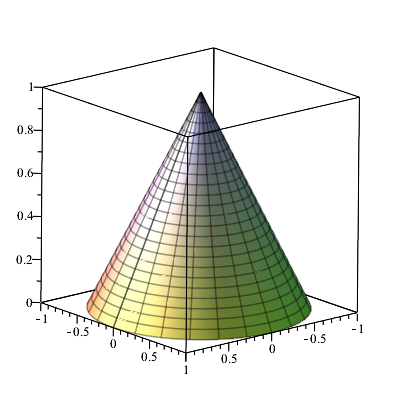
\includegraphics{11_8_Cylindrical_ex}}
  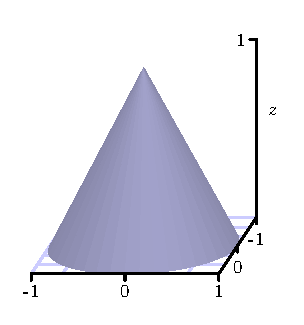
\includegraphics{figures/fig_11_8_cone.eps}
\end{center}
\caption{The cylindrical cone $r = 1-z$.}
\label{F:11.8.Cylindrical_ex}
\end{minipage} \hspace{0.5in}
\begin{minipage}{2.5in}
\begin{center}
%\resizebox{!}{2.4in}{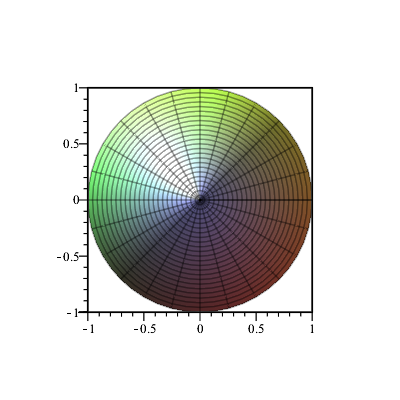
\includegraphics{11_8_Cylindrical_ex_proj}}
  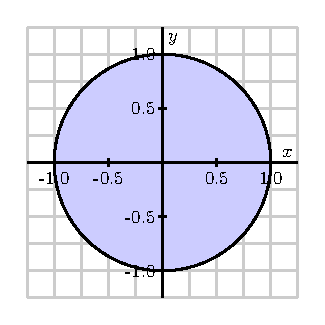
\includegraphics{figures/fig_11_8_cone_project.eps}
\end{center}
\caption{The projection into the $xy$-plane.}
\label{F:11.8.Cylindrical_proj}
\end{minipage}
\end{center}
\end{figure}

	\item Determine an iterated integral expression in cylindrical coordinates whose value is the volume of the solid bounded below by the cone $z = \sqrt{x^2+y^2}$ and above by the cone $z = 4 - \sqrt{x^2+y^2}$. A picture is shown in Figure \ref{F:11.8.Cylindrical_ex2}.
\begin{figure}[ht]
\begin{center}
%\resizebox{!}{2.75in}{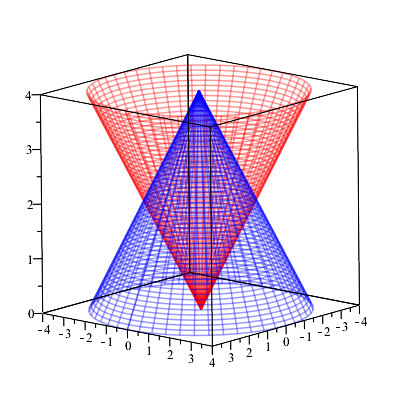
\includegraphics{11_8_Cylindrical_ex2}}
  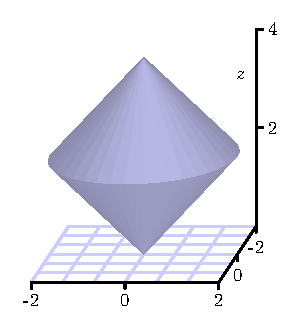
\includegraphics{figures/fig_11_8_two_cones.eps}
\end{center}
\caption{A solid bounded by the cones $z = \sqrt{x^2+y^2}$  and $z = 4 - \sqrt{x^2+y^2}$.}
\label{F:11.8.Cylindrical_ex2}
\end{figure}

\ea

\end{activity}
\begin{smallhint}

\end{smallhint}
\begin{bighint}

\end{bighint}
\begin{activitySolution}

\ba
\item Since $x^2+y^2=r^2$ in cylindrical coordinates, our limits on $z$ will be $0 \leq z \leq r^2$. Thus, an iterated integral in cylindrical coordinates that gives the volume of $S$ is  
\[\int \int \int_S 1 \, dV = \int_{0}^{2\pi} \int_0^1 \int_0^{r^2} (1) r \, dz \, dr \, d\theta.\]
Now
\begin{align*}
\int_{0}^{2\pi} \int_0^1 \int_0^{r^2} r \, dz \, dr \, d\theta &= \int_{0}^{2\pi} \int_0^1 \left. rz \right|_0^{r^2} \, dr \, d\theta \\
	&= \int_{0}^{2\pi} \int_0^1 r^3 \, dr \, d\theta \\
	&= \int_{0}^{2\pi} \left. \frac{r^4}{4} \right|_0^1 \, d\theta \\
	&= \frac{1}{4} \int_{0}^{2\pi} \, d\theta \\
	&= \frac{\pi}{2}.
\end{align*}

\item Recall that mass is the integral of density, so the mass of the cone is
\[\int \int \int_S \delta(r, \theta, z) \, dV.\]
The cone is bounded below by the $xy$-plane and above by the surface $r=1-z$. If we integrate with respect to $z$ first, then the limits on $z$ are $0 \leq z \leq 1-r$. When can project the surface into the $xy$-plane as shown in Figure \ref{F:11.8.Cylindrical_proj} to find the limits on $r$ and $\theta$. Note than when $z=0$ we have $r=1$, so the projection is a circle with radius centered at the origin. Therefore, the mass of the cone given the the iterated integral
\[\int \int \int_S \delta(r, \theta, z) \, dV = \int_0^{2\pi} \int_0^1 \int_0^{1-r} zr \, dz \, dr \, d\theta.\]

\item In cylindrical coordinates the cones are $z=r$ and $z=4-r$. So we have $r \leq z \leq 4-r$. Now $z=r$ and $z=4-r$ intersect when $r = 4-r$ or when $r=2$. So the projection of this solid in the $xy$-plane is the disk $0 \leq r \leq 2$ and $0 \leq \theta \leq 2\pi$. So an iterated integral in cylindrical coordinates that gives the volume of this solid is
\[\int_0^{2\pi} \int_0^2 \int_{r}^{4-r} r \, dz \, dr \, d\theta.\]

\ea

\end{activitySolution}
\aftera
